\chapter{Results}
\label{results}

\section{Dead projects}
\label{section:deads}
The data set of 250 projects was gathered in July 2013, and contains data points
up to June 2013.

A total of 38 (15.2\%) projects complied to the definition of a dead project as
defined in section \ref{def:dead}. Manual verification of the 38 potential
dead projects using the project's websites, source code repositories, and
commit history up to April 2014, revealed that 21 (8.4\%) are still complying
to the definition of a dead project in April 2014.

The 21 dead projects and their $age\_in\_months$ at the moment of death as a
result of the verification are shown in Table \ref{table:deads}.

\begin{wraptable}{l}{40mm}
\caption{Dead projects}\label{table:deads}
\centering
\begin{tabular}{rr}
  \hline
 ID & Died at month \\ 
  \hline
317799 &   2 \\ 
  587198 &   3 \\ 
  588411 &   5 \\ 
  589515 &   7 \\ 
  587204 &   8 \\ 
  585077 &   9 \\ 
  587571 &  11 \\ 
  586805 &  14 \\ 
  360279 &  30 \\ 
  322065 &  37 \\ 
  11389 &  46 \\ 
  12053 &  68 \\ 
  3085 &  71 \\ 
  307140 &  71 \\ 
  4614 &  75 \\ 
  41745 &  80 \\ 
  155830 &  84 \\ 
  325178 &  92 \\ 
  4007 & 120 \\ 
  15700 & 121 \\ 
  12547 & 142 \\  
   \hline
\end{tabular}
\end{wraptable}

\paragraph{}
All, except one, of the projects in Table \ref{table:deads} are dead because it
was abandoned by the community of contributors. Except for project with ID
587204, which is still receiving updates, but at very slow and sporadic
intervals. However, since the updates do not involve code activity, it is
considered dead.

\paragraph{}
When zooming in on the project with ID 317799, which is the youngest in this set
and died in its second month, it shows that this project has had a history of
the slightest change in its lines of code evolution. The project has had a total
number of 7 commits during the time it is being tracked by Ohloh (since
September 2011). A total of 4 contributors have worked on the project since it
was tracked. The most recent commit was done in October 2011.

\paragraph{}
Project with ID 12547 is the oldest. It died after 142 tracked months and has
had its most recent commits in February 2012. A total of 10 contributors have
worked on this project since May 2000.

\paragraph{}
The special case project, with ID 587204, is the only project that is not
abandoned by its (entire) community. The project has had 3 contributors over its
lifetime. One of them is still active every now and then. The most recent
commits were done in January 2014, the commits before that were in June 2012.
The commits involved updates in documentation, and the creation of a
configuration file for a continuous integration server. These commits do not
involve code changes.

The project died in July 2012, after 8 months since the first data point
tracked.

\paragraph{}
From the initial 38 projects, the remaining 17 projects complying to the
definition of dead (section \ref{def:dead}) appeared to be still alive. For 9
of the projects activity is very low or rapidly decreasing; 5 projects were
migrated to another source code repository; and for 3 projects the activity is
increasing after a long period of no activity.

\paragraph{}
The 9 projects with very low or decreasing activity show signs of 'dying'. Their
community is slowly but surely abandoning the project as can be seen by a
decrease of 35\% to 55\% of contributors, and/or commits.

The 5 migrated projects for which the tracking information is not updated at
Ohloh are lost. The tracking is stopped from the moment the project is
migrated. The tracking and analysis can be recovered by updating the source
code locations at Ohloh, but for this study the project is out of sight.

The 3 projects that have had no activity in a year, but after that show little
increase of activity are more difficult to explain. Manual evaluation showed
that there exist similar projects outside the data set that eventually die, but
there are also similar projects that eventually got 'resurrected'.



\section{Sequences and patterns}
The wavelet transform of the LOC signals of 250 projects resulted in 22,943
data points decomposed up to 7 levels into wavelet/shift and filter/scale
coefficients.

The similar sequence identification found 1,669,448 sequences that occurred
at least 2 times. A mere 16 sequences were found in wavelet/shift coefficients,
the other 1,669,432 sequences were found in filter/scale coefficients.

\paragraph{}
The second wavelet analysis step aggregated similar sequences across multiple
pairs together to form patterns. The detection of these 'popular sequences'
found 16,049 patterns. The patterns consist only of sequences of scale/filter
coefficients.

Some patterns that were found are shown in Figure \ref{figure:patterns_plots}.
The four graphs are plots of patterns recomposed onto the original signal. The
graphs all have multiple ($>$ 140) occurences of the pattern plotted of one or
more projects in the same graph. The graphs show that the sequences have
similar waveforms. Each graph contains a multiple of plotted sequences: pattern
1 contains 216 sequences; pattern 2 contains 156 sequences; pattern 3 contains
151 sequences; and pattern 4 contains 141 sequences.


\begin{figure}[H]
\caption{Example of a pattern found during wavelet
analysis}\label{figure:patterns_plots}
\centering
	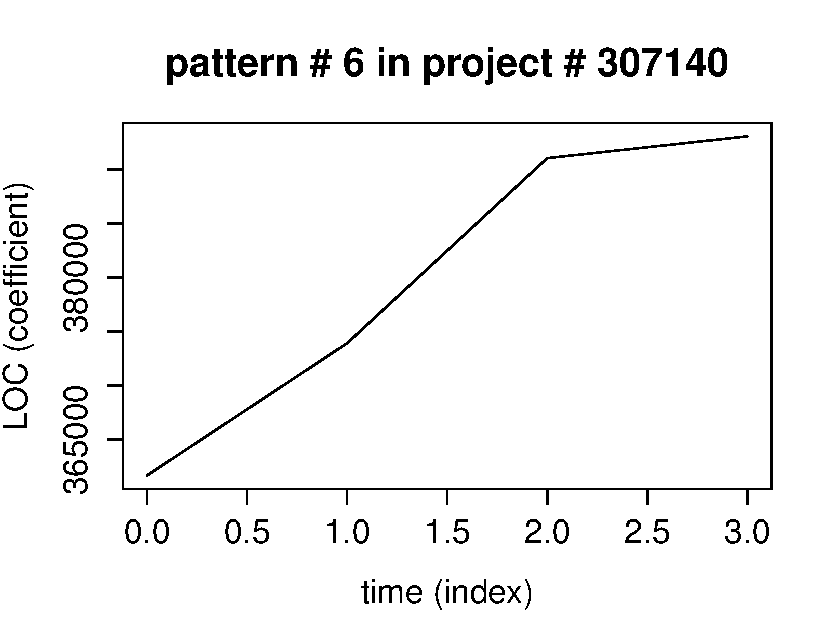
\includegraphics[width=196pt]{images/pattern_6.pdf}\\
	\vspace{1em}
	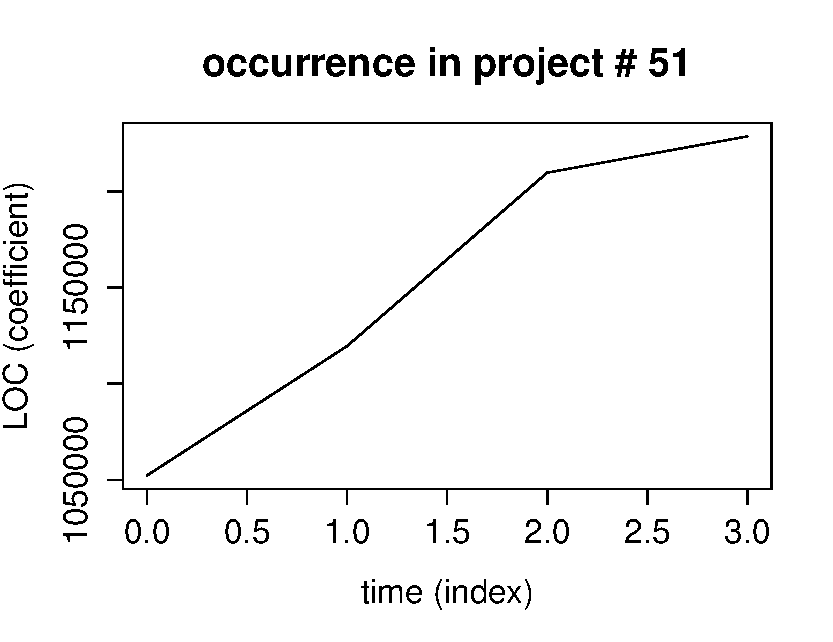
\includegraphics[width=128pt]{images/pattern_6_seq_e.pdf}
	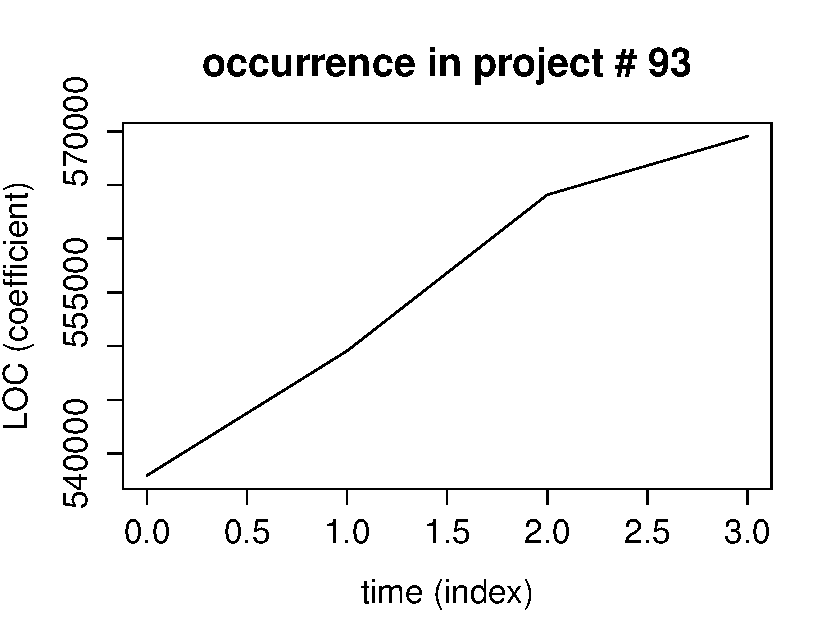
\includegraphics[width=128pt]{images/pattern_6_seq_d.pdf}
	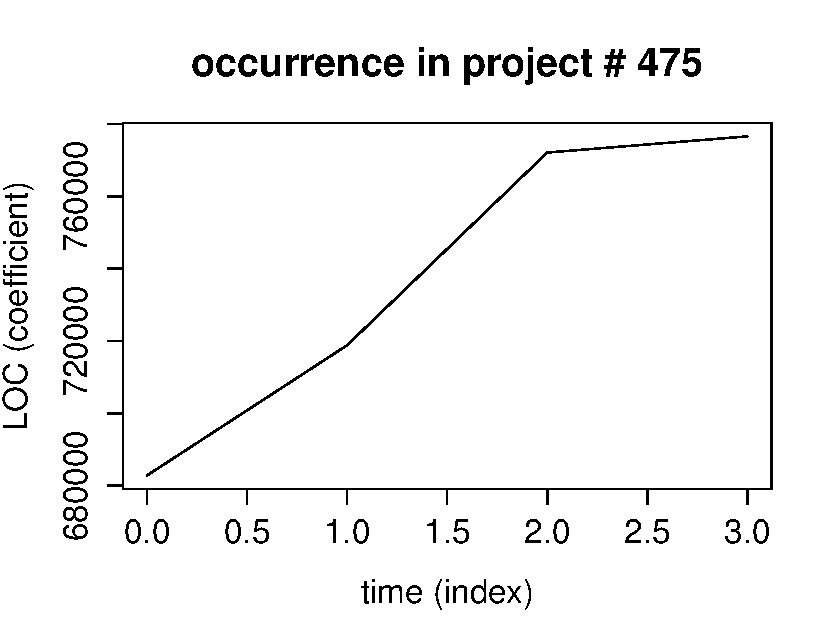
\includegraphics[width=128pt]{images/pattern_6_seq_c.pdf}
	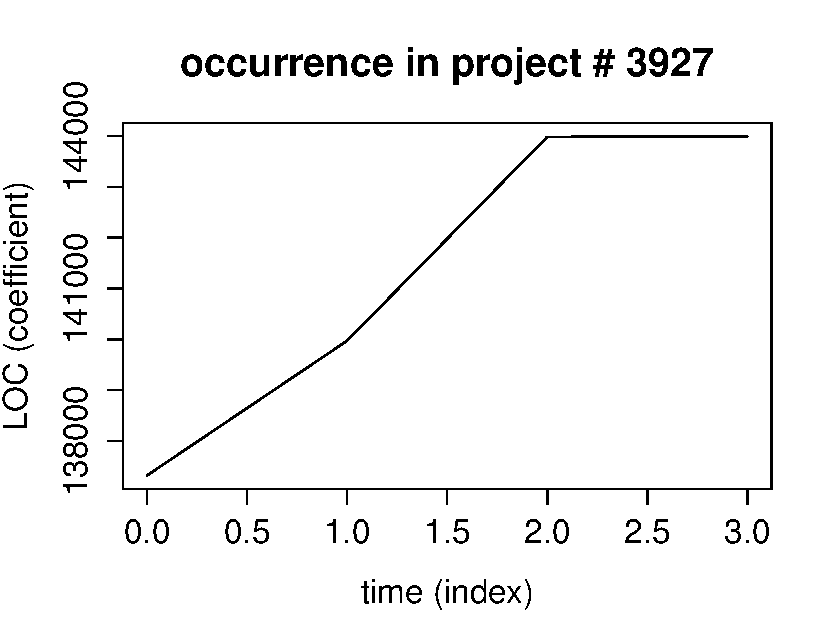
\includegraphics[width=128pt]{images/pattern_6_seq_f.pdf}
	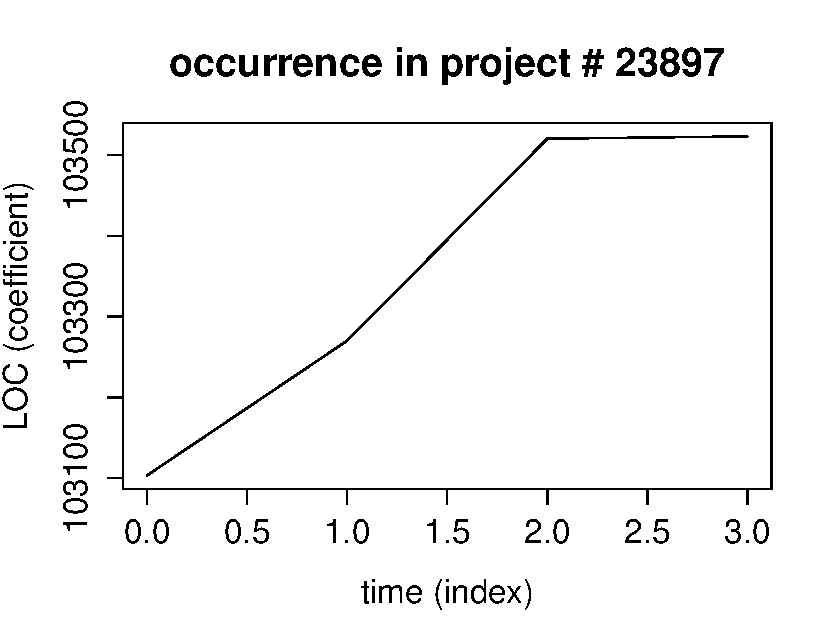
\includegraphics[width=128pt]{images/pattern_6_seq_a.pdf}
	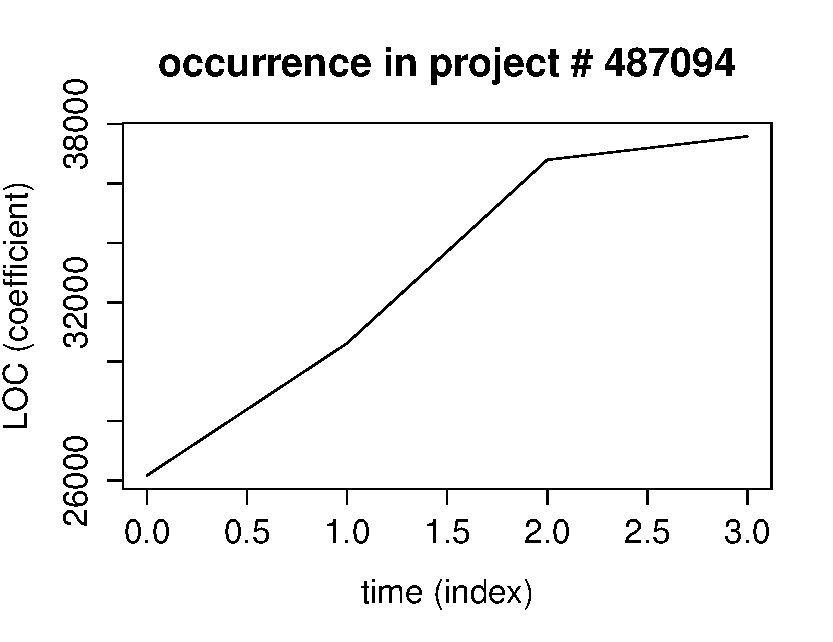
\includegraphics[width=128pt]{images/pattern_6_seq_b.pdf}
\end{figure}

\paragraph{}
The patterns occurred between 5 and 1,512 times across the projects. On
average, a pattern occurs 104 times. A single pattern occurs in at least 1 and
at most 204 projects (36 projects on average). The pattern length is between 4
and 19 coefficients (on average 6) across decomposition levels 3 to 7. The
higher the level, the closer the level of detail of the wavelet is to the
original signal.

\paragraph{}

12,643 (79\%) of the patterns appear in both dead and alive projects; 3,390
(21\%) of the patterns appear in alive projects only; and 16 (0.1\%) of the
patterns appear in dead projects only.

\section{Pattern classification}
The types of patterns from section \ref{section:patterns_dead} was the result
of identification of patterns in dead projects only. There were are total of
967 patterns found across 21 dead projects, of which 25 of type A, 317 of type
B, and 625 of type AB.

%\subsection{Patterns in dead projects}
%The patterns that were found in dead projects were typed as shown in section
%\ref{section:patterns_dead}.

\begin{comment}
- Factual results
- Tables and figures for clarification

This chapter presents and clarifies the results obtained during the research.
The focus should be on the factual results, not the interpretation or
discussion. Tables and graphics should be used to increase the clarity of the
results where applicable.
Have a look at the the results chapter in this example thesis on Paul’s
homepage\footnote{http://homepages.cwi.nl/~paulk/thesesMasterSoftwareEngineering/2006/ArnoldLankamp.pdf}.
\end{comment}
